\begin{frame}{Multi-Head Attention}
  \begin{itemize}
    \item[$\blacktriangleright$] Multi-head attention allows the model to jointly attend to information from different representation subspaces at different positions.
    \item[$\blacktriangleright$] It consists of multiple attention heads, each with its own set of parameters.
    \item[$\blacktriangleright$] The outputs of all heads are concatenated and linearly transformed.
  \end{itemize}

  \vspace{0.7em}

  \textbf{Formula:}
  \[
    \mathrm{MultiHead}(Q, K, V) = \mathrm{Concat}(\text{head}_1, \ldots, \text{head}_h) W^O
  \]
  where each head is defined as:
  \[
    \text{head}_i = \mathrm{Attention}(Q W_i^Q, K W_i^K, V W_i^V)
  \]

  \vspace{0.5em}
  \begin{itemize}
    \item[$\blacktriangleright$] $W_i^Q$, $W_i^K$, and $W_i^V$ are learned projection matrices for each head.
    \item[$\blacktriangleright$] $W^O$ is the output projection matrix that combines the outputs of all heads.
  \end{itemize}
\end{frame}

\begin{frame}{Multi-Head Attention} 
  \centering
  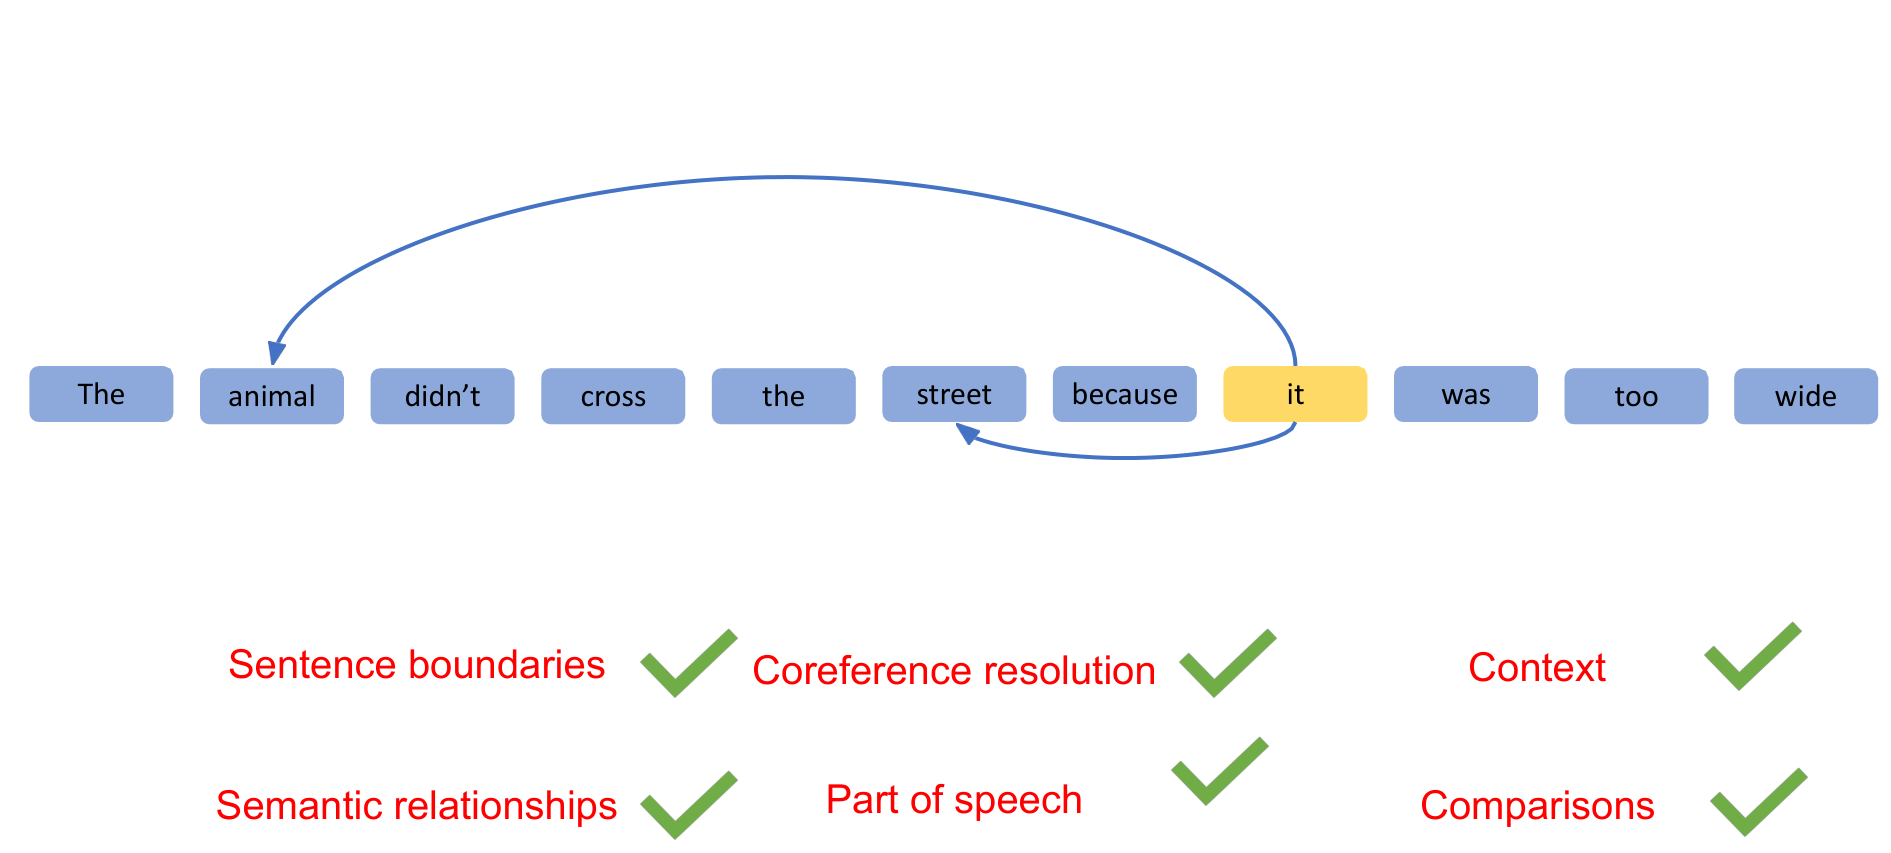
\includegraphics[width=0.9\paperwidth,height=0.95\paperheight,keepaspectratio]{images/introduction-to-transformers/transformer_nlp_tasks_all_solved_checkmarks.png}
\end{frame}

\begin{frame}{Multi-Head Attention} 
  \centering
  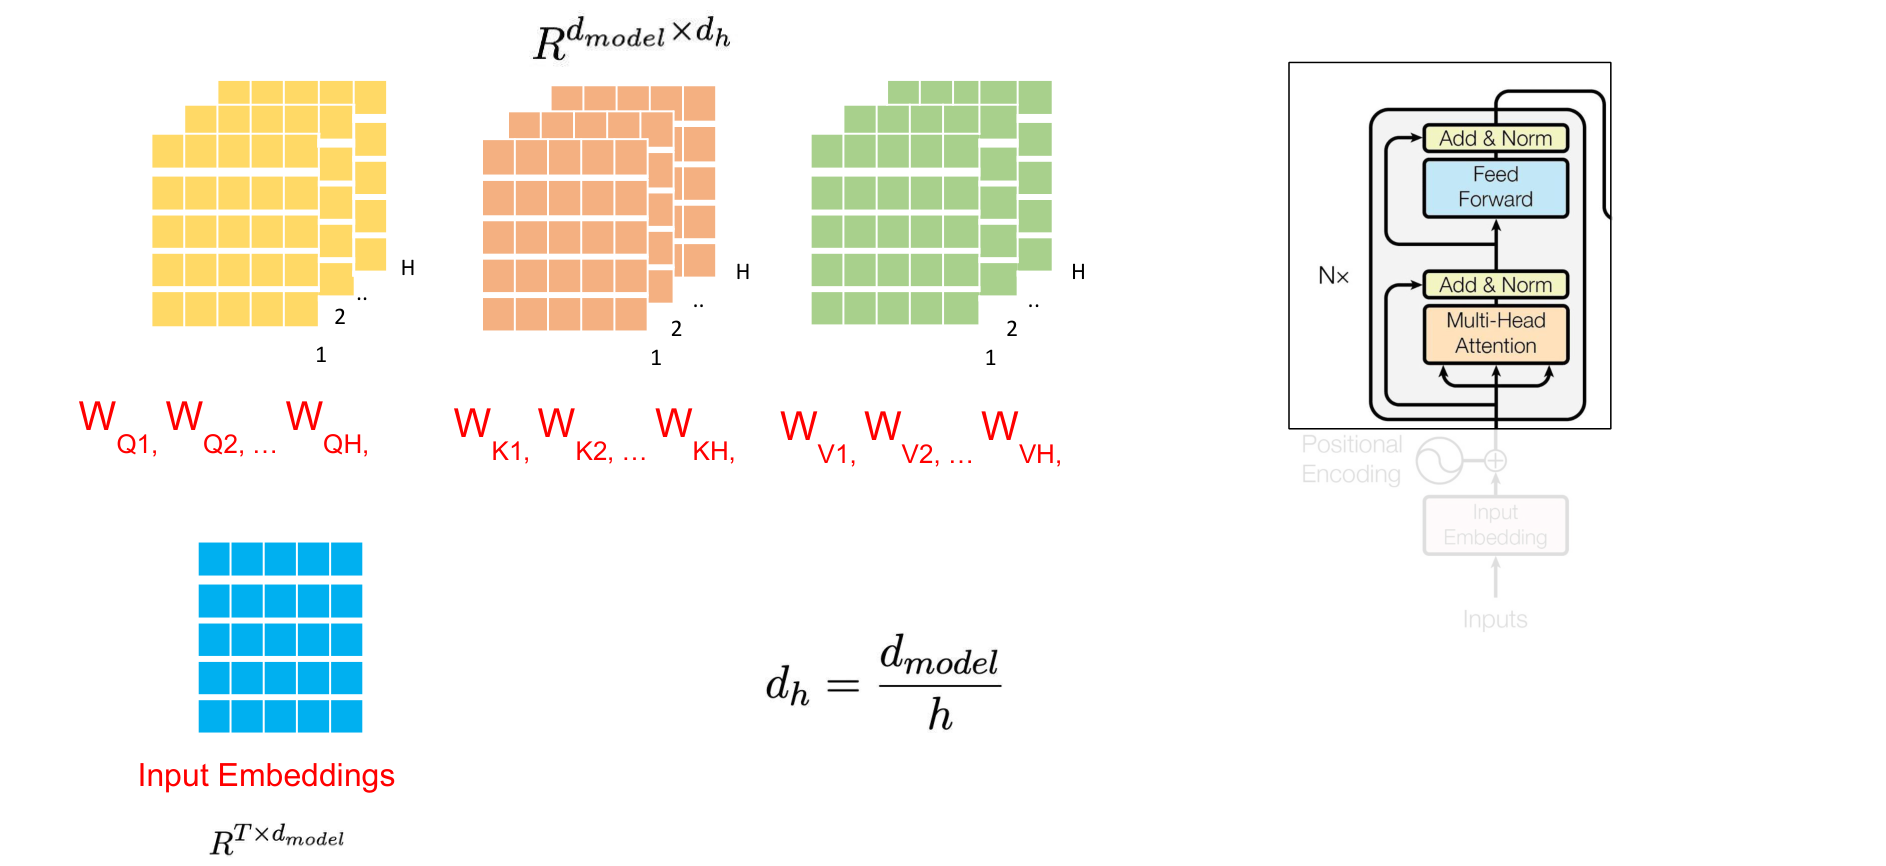
\includegraphics[width=0.9\paperwidth,height=0.95\paperheight,keepaspectratio]{images/introduction-to-transformers/transformer_multihead_stacked_weight_matrices_dh.png}
\end{frame}

\begin{frame}{Multi-Head Attention} 
  \centering
  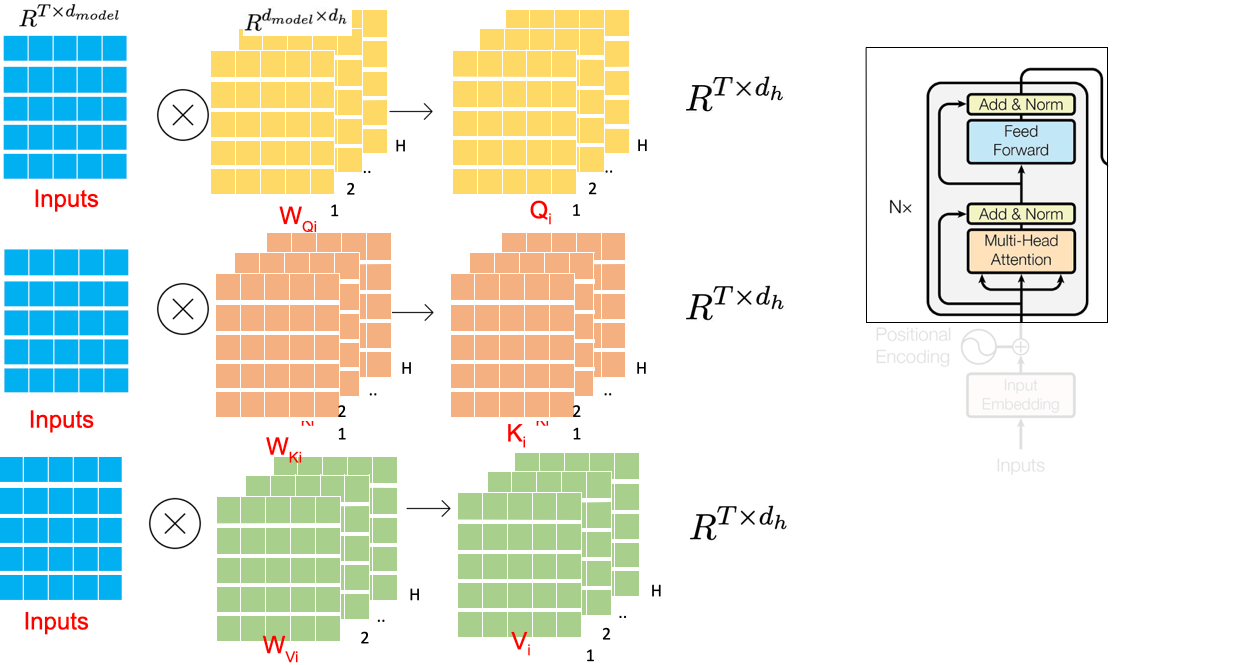
\includegraphics[width=0.9\paperwidth,height=0.95\paperheight,keepaspectratio]{images/introduction-to-transformers/transformer_multihead_qkv_projections_per_head.png}
\end{frame}

\begin{frame}{Multi-Head Attention} 
  \centering
  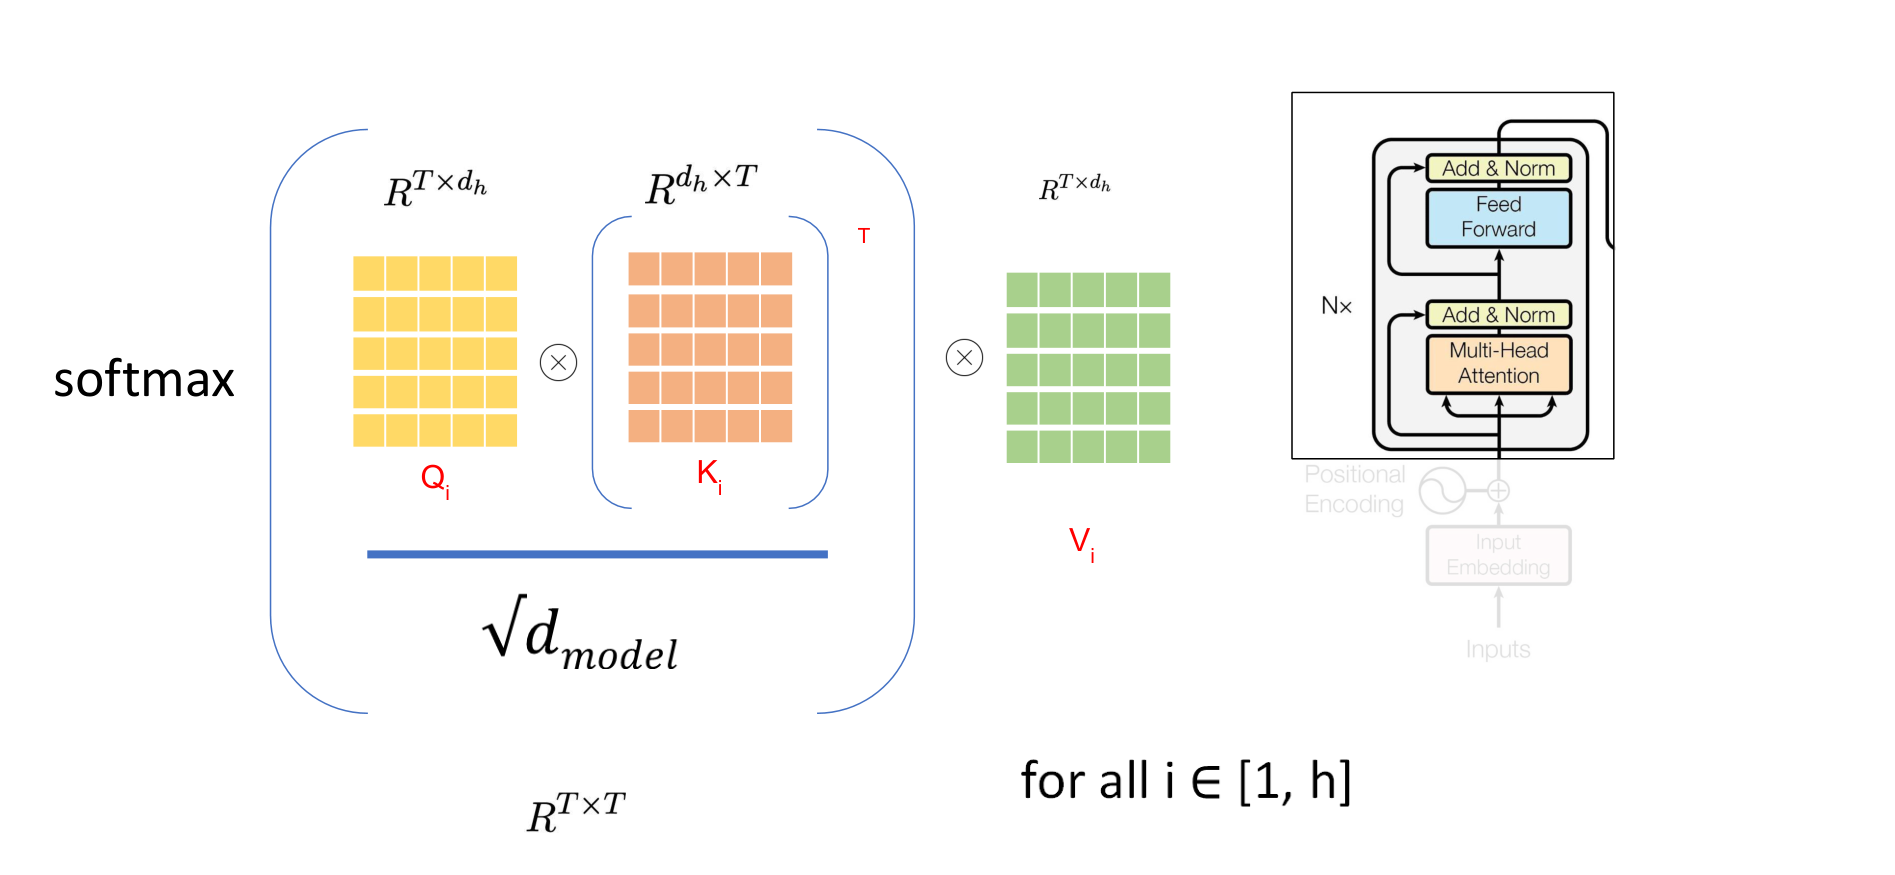
\includegraphics[width=0.9\paperwidth,height=0.95\paperheight,keepaspectratio]{images/introduction-to-transformers/transformer_multihead_softmax_attention_per_head.png}
\end{frame}

\begin{frame}{Multi-Head Attention} 
  \centering
  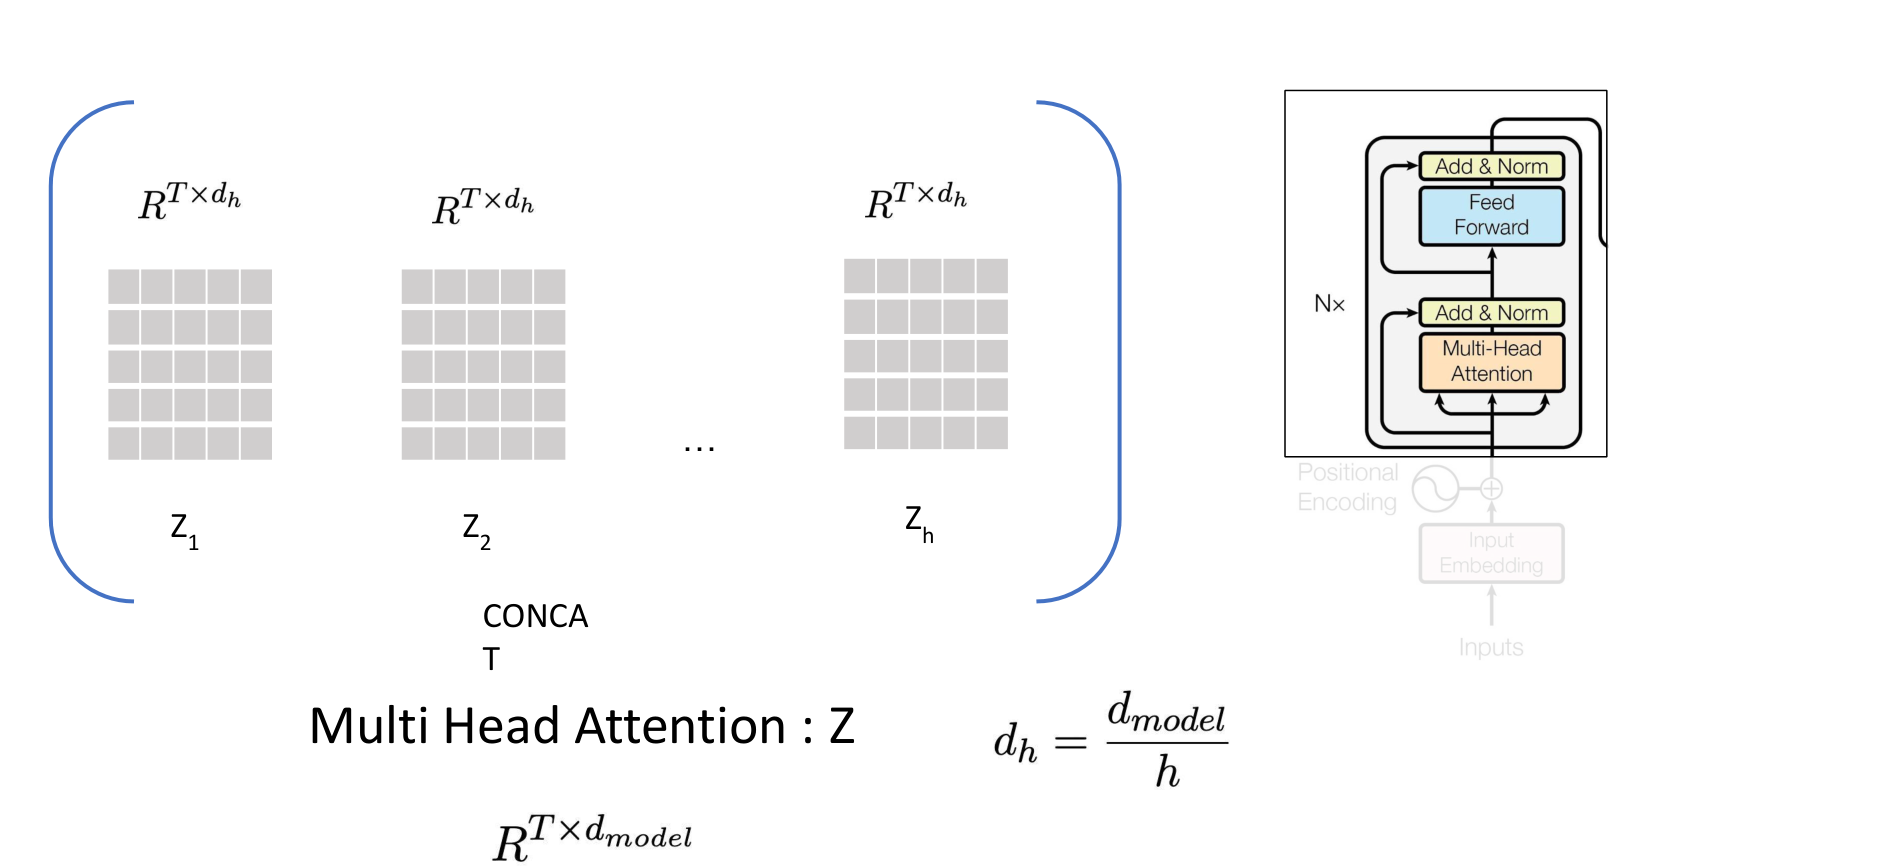
\includegraphics[width=0.9\paperwidth,height=0.95\paperheight,keepaspectratio]{images/introduction-to-transformers/transformer_multihead_concat_z_heads.png}
\end{frame}

\begin{frame}{Multi-Head Attention} 
  \centering
  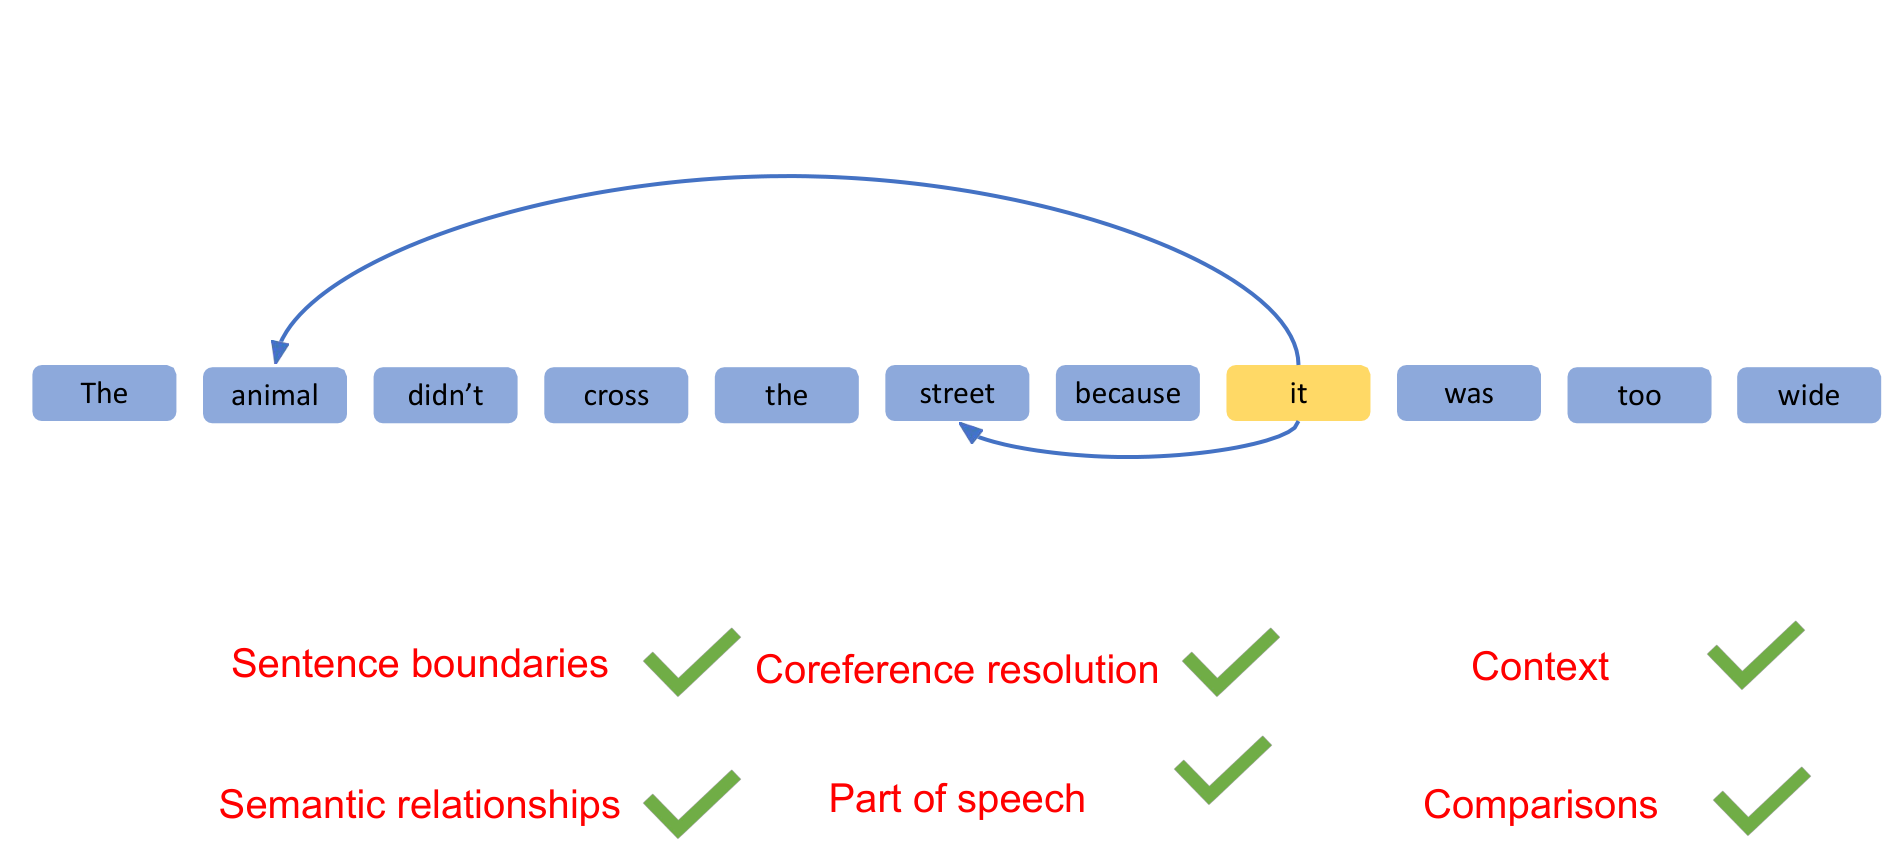
\includegraphics[width=0.9\paperwidth,height=0.95\paperheight,keepaspectratio]{images/introduction-to-transformers/transformer_nlp_tasks_all_solved_final.png}
\end{frame}

\begin{frame}{Benefits of Multi-Head Attention}
  \begin{itemize}
    \item[$\blacktriangleright$] Enables the model to jointly attend to information from different representation subspaces at different positions.
    \item[$\blacktriangleright$] Captures various linguistic and syntactic patterns by using multiple attention heads.
    \item[$\blacktriangleright$] Improves the model's ability to represent complex relationships in the data.
    \item[$\blacktriangleright$] Provides richer and more diverse feature representations.
  \end{itemize}
\end{frame}

